\documentclass[12t,letterpaper]{article}

\newenvironment{proof}{\noindent{\bf Proof:}}{\qed\bigskip}

\newtheorem{theorem}{Theorem}
\newtheorem{corollary}{Corollary}
\newtheorem{lemma}{Lemma} 
\newtheorem{claim}{Claim}
\newtheorem{fact}{Fact}
\newtheorem{definition}{Definition}
\newtheorem{assumption}{Assumption}
\newtheorem{observation}{Observation}
\newtheorem{example}{Example}
\newcommand{\qed}{\rule{7pt}{7pt}}

\newcommand{\assignment}[4]{
\thispagestyle{plain} 
\newpage
\setcounter{page}{1}
\noindent
\begin{center}
\framebox{ \vbox{ \hbox to 6.28in
{\bf EE 126: Probability and Random Processes \hfill #1}
\vspace{4mm}
\hbox to 6.28in
{\hspace{2.5in}\large\mbox{#2}}
\vspace{4mm}
\hbox to 6.28in
{{\it Handed Out: #3 \hfill Due: #4}}
}}
\end{center}
}

\newcommand{\solution}[3]{
\thispagestyle{plain} 
\newpage
\setcounter{page}{1}
\noindent
\begin{center}
\framebox{ \vbox{ \hbox to 6.28in
{\bf EE 126 \hfill #3}
\vspace{4mm}
\hbox to 6.28in
{\hspace{2.5in}\large\mbox{#2}}
\vspace{4mm}
\hbox to 6.28in
{#1 \hfill}
}}
\end{center}
\markright{#1}
}

\newenvironment{algorithm}
{\begin{center}
\begin{tabular}{|l|}
\hline
\begin{minipage}{1in}
\begin{tabbing}
\quad\=\qquad\=\qquad\=\qquad\=\qquad\=\qquad\=\qquad\=\kill}
{\end{tabbing}
\end{minipage} \\
\hline
\end{tabular}
\end{center}}

\def\Comment#1{\textsf{\textsl{$\langle\!\langle$#1\/$\rangle\!\rangle$}}}


\usepackage{amsmath, dsfont, mathtools, verbatim, tikz, float}

\usetikzlibrary{arrows,automata}

\oddsidemargin 0in
\evensidemargin 0in
\textwidth 6.5in
\topmargin -0.5in
\textheight 9.0in

\newenvironment{amatrix}[1]{%
  \left(\begin{array}{@{}*{#1}{c}|c@{}}
}{%
  \end{array}\right)
}

\DeclarePairedDelimiter{\ceil}{\lceil}{\rceil}
\DeclareMathOperator*{\argmin}{arg\,min}
\DeclareMathOperator*{\argmax}{arg\,max}

\makeatletter
\renewcommand*\env@matrix[1][*\c@MaxMatrixCols c]{%
  \hskip -\arraycolsep
  \let\@ifnextchar\new@ifnextchar
  \array{#1}}
\makeatother

\newcommand{\norm}[1]{\left\lVert #1 \right\rVert}
\newcommand{\abs}[1]{\left\vert #1 \right\vert}
\newcommand{\cov}[2]{\text{cov}(#1,#2)}
\newcommand{\var}[1]{\text{var}(#1)}
\newcommand{\?}{\stackrel{?}{=}}
\newcommand\given[1][]{\:#1\vert\:}
\renewcommand{\d}[1]{\ensuremath{\operatorname{d}\!{#1}}}

\begin{document}

\solution{Nikhil Unni}{HW11}{Spring 2016}
\pagestyle{myheadings}

\begin{enumerate}
  \item If $X = 0, Y = U[-1,1]$ and if $X=1, Y = U[0,2]$. Solve a hypothesis testing problem so that the probability of false alarm is less than or equal to $\beta$.\\\\

    First we can find the likelihood function:
    $$L(-1 \leq y < 0) = \frac{0}{1} = 0$$
    $$L(0 \leq y \leq 1) = \frac{1}{1} = 1$$
    $$L(1 \leq y \leq 2) = \infty$$
    
    We want to pick a $\lambda, \gamma$ such that $P(L(y) = \lambda | X = 0)(\gamma) = \beta$. Since we're conditioned on $X=0$, $L(y)$ cannot be $\infty$. If we pick $\lambda = 0$ (or $\lambda = 1$, really), we get:
    $$P(L(y) = \lambda | X=0)(\gamma) = \beta$$
    $$\frac{1}{2}(\gamma) = \beta$$
    $$\gamma = 2 \beta$$
  \item The random variables $X,Y,Z$ are i.i.d. $N(0,1)$.\\\\

    First let's find a few probabilities:
    $$E[X] = E[Y] = E[Z] = 0$$
    $$E[X^2] = E[Y^2] = E[Z^2] = \mu^2 + \sigma^2 = 1$$
    $$E[X^3] = E[Y^3] = E[Z^3] = \mu(\mu^2 + 3 \sigma^2) = 0$$
    \begin{enumerate}
      \item Find $L[X^2 + Y^2 | X + Y]$\\\\
        
        From the definition of LLSE, we know:
        $$L[X^2 + Y^2 | X + Y] = E[X^2 + Y^2] + \frac{\cov{X^2+Y^2}{X+Y}}{\var{X+Y}}(X+Y - E[X+Y])$$
        And $\cov{X^2+Y^2}{X+Y} = E[(X^2+Y^2)(X+Y)] - E[X^2+Y^2]E[X+Y]$. The second expression is $0$, since $E[X]=E[Y]=0$, and so then we have:
        $$\cov{X^2+Y^2}{X+Y} = E[(X^2+Y^2)(X+Y)] = E[X^3] + E[X^2Y] + E[XY^2] + E[Y^3] = 0 + 0 + 0 + 0$$

        So then we have:
        $$L[X^2 + Y^2 | X + Y] = E[X^2] + E[Y^2] = 2$$

      \item Find $L[X + 2Y | X + 3Y + 4Z]$\\\\

        From the definition of LLSE, we know:
        $$L[X+2Y | X+3Y+4Z] = E[X+2Y] + \frac{\cov{X+2Y}{X+3Y+4Z}}{\var{X+3Y+4Z}}(X+3Y+4Z - E[X+3Y+4Z])$$

        And: 
        $$\cov{X+2Y}{X+3Y+4Z} = E[X^2+3XY+4XZ+2XY+6Y^2+8YZ^2] - E[X+2Y]E[X+3Y+4Z] = (1+6) - 0 = 7$$
        And:
        $$\var{X+3Y+4Z} = \var{X} + 9\var{Y} + 16\var{Z} = 1+9+16 = 26$$

        So we have:
        $$L[X^2 + Y^2 | X + Y] = \frac{7}{26}(X+Y)$$        

      \item Find $L[(X+Y)^2 | X-Y]$\\\\

        From the definition of LLSE, we know:
        $$L[(X+Y)^2 | X-Y] = E[(X+Y)^2] + \frac{\cov{(X+Y)^2}{X-Y}}{\var{X-Y}}(X-Y-E[X-Y])$$
        $$=E[(X+Y)^2] + \frac{E[(X+Y)(X^2-Y^2)] - E[(X+Y)^2]E[X-Y]}{E[(X-Y)^2] - E[X-Y]^2}$$

        We first have to find the expectations:
        $$E[(X+Y)^2] = E[X^2] + 2E[XY] + E[Y^2] = 1 + 0 + 1 = 2$$
        $$E[(X+Y)^2(X-Y)] = E[X^3] + E[X^2Y] - E[XY^2] - E[Y^3] = 0 + 0 + 0 + 0 = 0$$

        Since both $E[(X+Y)^2(X-Y)]$ and $E[X-Y]$ are $0$, the entire fraction is $0$. Meaning we have:
        $$L[(X+Y)^2 | X-Y] = 2$$
    \end{enumerate}


  \item Consider a photodetector in an optical communications system that counts the number of photons arriving during a certain interval. A user conveys information by switching a photon transmitter on or off. Assume that the probability of the transmitter being on is $p$. If the transmitter is on, the number of photons transmitted over the interval of interest is a Poisson random variable $\theta$ with mean $\lambda$ and if it is off, the number of photons transmitted is $0$. Unfortunately, regardless of whether or not the transmitter is on or off, photons may be detected due to ``shot noise''. The number $N$of detected shot noise photons is a Poisson random variable $N$ with mean $\mu$. Given the number of detected photons, find the LLSE of the number of transmitted photons.\\\\

    Let's call the number of transmitted photons $X$, and call the number of detected photons $Y$. Let $T$ be the random variable denoting whether or not the transmitter is on. $T=1$ with probability $p$, and $T=0$ with probability $1-p$. So then we know:
    $$X = T \theta$$
    $$Y = X + N$$
    We want to find $L[X|Y]$. From our LLSE formula, we know this is:
    $$L[X|Y] = E[X] + \frac{\cov{X}{Y}}{\var{Y}}(Y - E[Y])$$
    $$=E[X] + \frac{E[XY] - E[X]E[Y]}{E[Y^2] - E[Y]^2}(Y - E[Y])$$

    Calculating all the necessary probabilities:
    $$E[X] = E[T] E[\theta] = p \lambda$$
    $$E[Y] = E[X] + E[N] = p \lambda + \mu$$
    $$E[X^2] = pE[\theta^2] + (1-p)*0 = p(\lambda^2 + \lambda)$$
    $$E[XN] = E[X]E[N] = p \lambda \mu$$
    $$E[Y^2] = E[X^2] + 2E[XN] + E[N^2] = p(\lambda^2 + \lambda) + 2p \lambda \mu + (\mu^2 + \mu)$$
    $$E[XY] = E[X^2 + XN] = p(\lambda^2 + \lambda) + 2p \lambda \mu$$

    So putting it all together, we get:
    $$L[X|Y] = p \lambda + \frac{p \lambda^2 + p \lambda + 2p \lambda \mu - p \lambda(p \lambda + \mu)}{p(\lambda^2 + \lambda) + 2p \lambda \mu + \mu^2 + \mu - p^2 \lambda^2 - 2 p \lambda \mu - \mu^2}(Y - p \lambda - \mu)$$
    $$=p \lambda + \frac{p \lambda^2 + p \lambda + p \lambda \mu - p^2 \lambda^2}{p \lambda^2 + p \lambda + \mu - p^2 \lambda^2}(Y - p \lambda - \mu)$$

  \item Let $(V_n, n \geq 0)$ be i.i.d. $N(0, \sigma^2)$ and independent of $X_0 = N(0,u^2)$. Define
    $$X_{n+1} = aX_n + V_n, n \geq 0$$
    \begin{enumerate}
      \item What is the distribution of $X_n$ for $n \geq 1$?\\\\

        Looking at the terms, we have:
        $$X_0 = N(0, u^2)$$
        $$X_1 = N(0, a^2u^2) + N(0, \sigma^2) = N(0, a^2u^2 + \sigma^2)$$
        $$\cdots$$

        So we can create a recurrence relation on the variance at step $n$:
        $$T(0) = u^2, T(n) = a^2 T(n-1) + \sigma^2$$
        Solving, we get:
        $$T(n) = \frac{a^{2n}(a^2u^2 - u^2 + \sigma^2) - \sigma^2}{a^2 - 1}$$

        So we have $X_n \sim N(0, \frac{a^{2n}(a^2u^2 - u^2 + \sigma^2) - \sigma^2}{a^2 - 1})$.

      \item Find $E[X_{n+m} | X_n]$ for $0 \leq n < n + m$.\\\\

        Given $X_n$, we know that:
        $$X_{n+1} = aX_n + N(0,\sigma^2) = N(aX_n,\sigma^2)$$
        $$X_{n+2} = aN(aX_n, \sigma^2) + N(0, \sigma^2) = N(a^2X_n, a^2 \sigma^2 + \sigma^2)$$
        $$\cdots$$

        In general, we know that that $X_{m \geq n}$ will be normally distributed with mean $a^{m-n} X_n$. So then, clearly:
        $$E[X_{n+m} | X_n] = a^m X_n$$

      \item Find $u$ so that the distribution of $X_n$ is the same for all $n \geq 0$.\\\\

        We know that the mean of the $X_n$ are all $0$. So we want the variances to be all the same. Looking at the closed formula for the variance of $X_n$, we have:
        $$\frac{a^{2n}(a^2u^2 - u^2 + \sigma^2) - \sigma^2}{a^2-1}$$
        The only way to make this a constant is to remove the $a^{2n}$ term, by finding a value of $u$ such that:
        $$a^2u^2 - u^2 + \sigma^2 = 0$$
        Rearranging and solving for $u$:
        $$u^2(a^2 - 1) + \sigma^2 = 0$$
        $$u = \frac{\sigma}{\sqrt{1-a^2}}$$
    \end{enumerate}
  \item The difficulty of an EE126 exam, $\theta$, is uniformly distributed on $[0,100]$, and Alice gets a score $X$ that is uniformly distributed on $[0,\theta]$. Alice gets her score back and wants to estimate the difficulty of the exam.
    \begin{enumerate}
      \item What is the LLSE for $\theta$?\\\\

        $$LLSE[\theta | X] = E[\theta] + \frac{\cov{X}{\theta}}{\var{X}}(X - E[X])$$
        $$=E[\theta] + \frac{E[X \theta] - E[X]E[\theta]}{E[X^2] - E[X]^2}(X - E[X])$$

        First, we have to solve for those expectations:
        $$E[X] = E[E[X | \theta]] = E[\frac{\theta}{2}] = 25$$
        $$E[\theta^2] = \var{\theta} + E[\theta^2] = \frac{1}{12}(100^2) + 50^2 = \frac{10000}{3}$$
        $$E[X \theta] = E[E[X \theta | \theta]] = E[\theta(\frac{\theta}{2})] = \frac{1}{2}E[\theta^2] = \frac{5000}{3}$$
        $$E[X^2] = E[E[X^2 | \theta]] = E[\frac{1}{12}(\theta)^2 + (\frac{\theta}{2})^2] = \frac{1}{12}E[\theta^2] + \frac{1}{4}E[\theta^2] = \frac{10000}{9}$$

        So putting it all together:
        $$LLSE[\theta | X] = 50 + \frac{5000/3 - 25*50}{10000/9 - 25*25}(X - 25) = 50 + \frac{6}{7} (X - 25)$$

      \item What is the MAP of $\theta$?\\\\
        
        $$MAP[\theta | X] = \argmax_{\theta \geq X} P(X | \theta)$$
        $$=\argmax_{\theta \geq X} \frac{1}{\theta}$$
        $$=\argmin_{\theta \geq X} \theta = X$$

        So the $MAP$ decision would be $\min{X, 100}$, since $\theta$ is upper bounded by $100$.
        
      \item Find the mean squared error of each estimate as a function of the score $X$.

    \end{enumerate}
  \item The situation is the same as in the previous problem.
    \begin{enumerate}
      \item What is the MMSE of $\theta$ given $X$?\\\\

        $$MMSE[\theta|X] = E[\theta | X] = \int_{\theta} \theta \frac{f_{\theta}(\theta) f_{X|\theta}(X | \theta)}{f_{X}(X)} \d \theta$$
        Finding $f_X(x)$:
        $$f_X(x)= \int_{\theta} P(\theta)P(x | \theta) \d \theta$$
        Since $\theta \geq X$, we change the limits of integration accordingly:
        $$f_X(x) = \int_{\theta=X}^{100} \frac{1}{100} \frac{1}{\theta} \d \theta = \frac{1}{100}(\ln(100/x))$$
        So then we have:
        $$MMSE[\theta|X] = \int_{\theta=X}^{100} \theta \frac{\frac{1}{100}\frac{1}{\theta}}{\frac{1}{100} \ln(100/x)} \d \theta$$
        $$= \int_{\theta=X}^{100} \frac{1}{\ln(100/x)} \d \theta = \frac{100-X}{\ln(\frac{100}{X})}$$ 
      \item Plot the MAP, LLSE, and MMSE as a function of the score $X$.\\\\
        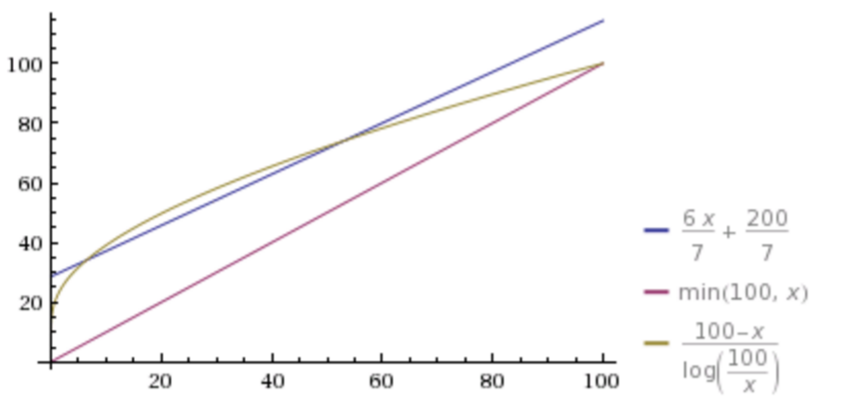
\includegraphics[width=1\textwidth]{img}
      \item Find the mean squared error of the MMSE as a function of the score $X$. Plot it along with the mean squared error of the MAP and LLSE.
        
    \end{enumerate}
  \item Let the joint density of two random variables $X$ and $Y$ be 
    $$f_{X,Y}(x,y) = \frac{1}{4}(2x+y), 0 \leq x \leq 1, 0 \leq y \leq 2$$
    First show that this is a valid joint distribution. Suppose you observe $Y$ drawn from this joint density. Find MMSE$[X|Y]$.\\\\

    We can show it's a valid distribution by integrating through $x$ and $y$:
    $$\int_{x=0}^1 \int_{y=0}^2 \frac{1}{4}(2x+y) \d y \d x$$
    $$= \frac{1}{4} \int_{x=0}^1 [2xy + \frac{y^2}{2}]_{y=0}^2 \d x = \frac{1}{4} \int_{x=0}^1 4x + 2 \d x$$
    $$= \frac{1}{4} [2x^2 + 2x]_{x = 0}^1 = \frac{1}{4}(2+2) = 1$$\\

    To find $E[X|Y]$, we first must find $f_{X|Y}(x|y) = \frac{f_{X,Y}(x,y)}{f_Y(y)}$. And:
    $$f_Y(y) = \int_{x=0}^1 \frac{1}{4}(2x+y) dx = \frac{1}{4}[x^2 + xy]_{x=0}^1 = \frac{1}{4}(1+y)$$
    And so:
    $$f_{X|Y}(x|y) = \frac{\frac{1}{4}(2x+y)}{\frac{1}{4}(1+y)} = \frac{2x+y}{1+y}$$

    Finally:
    $$E[X|Y] = \int_{x=0}^1 \frac{2x+y}{1+y} x = \frac{1}{1+y} [\frac{2}{3}x^3 + \frac{y}{2}x^2]_{x=0}^1 = \frac{3y+4}{6y+6}$$

  \item Let $X,Y,Z$ be three random variables. Prove formally that
    $$E[|X - E[X|Y]|^2] \geq E[|X - E[X|Y,Z]|^2]$$
    What is the intuition behind the inequality?\\\\

    $$E[(X - E[X|Y])^2] \geq E[(X - E[X|Y,Z])^2]$$
    Using the proof of Lemma 7.6(a) from Walrand:
    $$E[X^2] - 2E[X|Y]E[X] + E[X|Y]^2 \geq E[X^2] - 2E[X|Y,Z]E[X] + E[X|Y,Z]^2$$
    $$E[X|Y]^2 - 2E[X|Y]E[X] \geq E[X|Y,Z]^2 - 2E[X|Y,Z]E[X]$$

    The intution is that, with more information, Z, that our ``educated guess'' $E[X|Y,Z]$ can only be closer to the actual value of $X$ than our ``educated guess'' with only the information of Y, $E[X|Y]$. $Z$ may not help getting closer to $X$, but it cannot possibly move us farther away from the actual value of $X$.\\

    
\end{enumerate}

\end{document}
